\begin{center}
	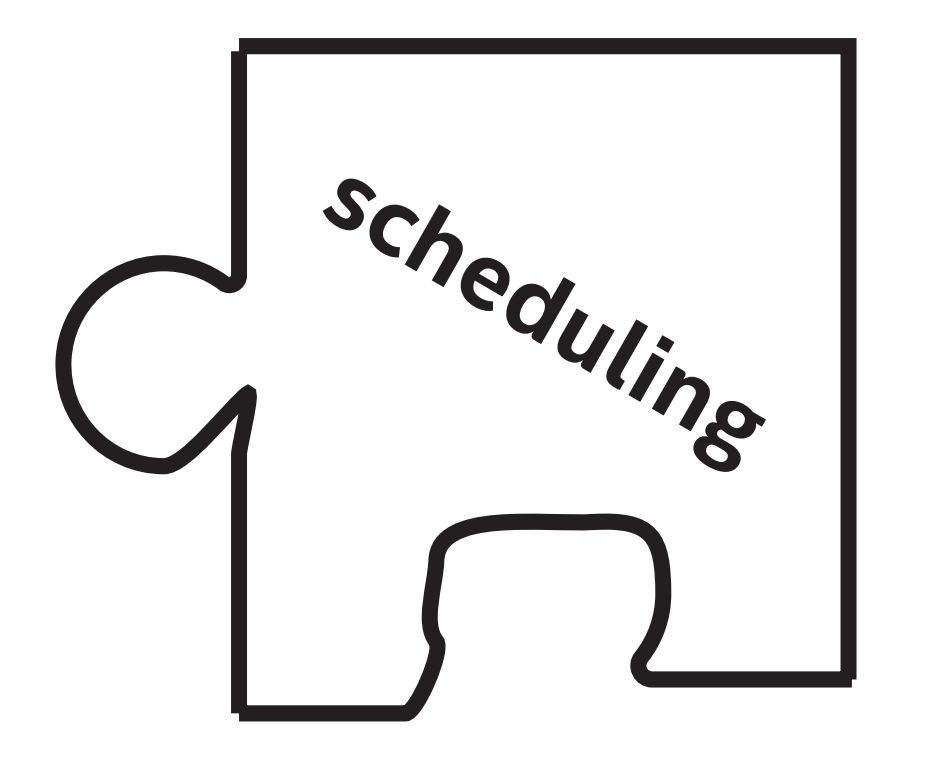
\includegraphics[width=0.3\textwidth]{content/chapter-8/images/1}
\end{center}

We need to discuss our role as the concert master for our parallel programs. The proper orchestration of a parallel program is a thing of beauty—code running full speed without waiting for data, because we have arranged for all data to arrive and depart at the proper times. Code well-decomposed to keep the hardware maximally busy. It is the thing that dreams are made of!\par

Life in the fast lanes—not just one lane!—demands that we take our 
work as the conductor seriously. In order to do that, we can think of our job in terms of task graphs.\par

Therefore, in this chapter, we will cover task graphs, the mechanism that is used to run complex sequences of kernels correctly and efficiently. There are two things that need sequencing in an application: kernels and data movement. Task graphs are the mechanism that we use to achieve proper sequencing.\par

First, we will quickly review how we can use dependences to order tasks from Chapter 3. Next, we will cover how the DPC++ runtime builds graphs. We will discuss the basic building block of DPC++ graphs, the command group. We will then illustrate the different ways we can build graphs of common patterns. We will also discuss how data movement, both explicit and implicit, is represented in graphs. Finally, we will discuss the various ways to synchronize our graphs with the host.\par